\documentclass[11pt]{article}

\usepackage[margin=1in]{geometry}
\usepackage{amsmath,amssymb,amsthm,bm}
\usepackage{booktabs,array}
\usepackage{siunitx}
\usepackage{pgfplots}
\usepackage{algorithm}
\usepackage{algpseudocode}
\usepackage{csquotes}
\usepackage{microtype}
\usepackage{hyperref}
\usepackage[capitalise,noabbrev]{cleveref}
\pgfplotsset{compat=1.18}
\hypersetup{colorlinks=true,linkcolor=black,citecolor=black,urlcolor=blue!50!black}

\newcommand{\R}{\mathbb{R}}
\newcommand{\softmax}{\operatorname{softmax}}
\newcommand{\LN}{\operatorname{LN}}
\newcommand{\GELU}{\operatorname{GELU}}
\newcommand{\MHA}{\operatorname{MHA}}
\newcommand{\code}[1]{\texttt{#1}}

\title{BibleLM: Retrieval, Graph Methods and a From-Scratch\\Language Model in an Offline Study Bible}
\author{Ryan Wetzstein}
\date{November 2026 \quad (describes v2.1.0)}

\begin{document}
\maketitle

\begin{abstract}
BibleLM is a desktop study Bible with a machine-learning laboratory inside it.
Its design rule is that \enquote{the machine finds, Scripture speaks}: every
learned component returns real verses with their references, and generated text
is always labelled and kept apart from the text of the Bible. This paper sets out
the mathematics behind each component. Semantic search scans $39{,}904$
verse embeddings ($384$ dimensions, $8$-bit), smooths scores across neighbouring
verses, and merges exact and semantic results by reciprocal rank fusion. On a
$30$-question benchmark, a bounded reranking judgment raises MRR@10 from $0.32$
to $0.55$ and nDCG@10 from $0.33$ to $0.55$. A graph of about $341{,}000$ cross
references supports personalized PageRank study walks and strongest-chain paths.
Corpus statistics (tf-idf, pointwise mutual information, Zipf's law, Burrows'
Delta and a null model for equidistant letter sequences) run in the client. The
Lab trains a character-level decoder-only transformer of about $10.8$M
parameters, with attention maps, a logit lens and per-verse surprise. Verse
memorization uses the FSRS-4.5 scheduler, and illustrations are dithered with
four classical halftoning algorithms.
\end{abstract}

\tableofcontents

\section{Design principles}\label{sec:principles}

Three constraints shape every method below.
\begin{description}
  \item[Retrieval over generation] Search, ranking and routing return indices
        into the canonical text; they never produce verse text.
  \item[Rules stay in code] References, counts, exact search and a book's
        genre are deterministic. A learned model may only order, filter or
        route.
  \item[Offline by default] Study features run in the client with no Python
        and no server. The only network call is an optional bounded judgment
        service, off unless the user supplies a key.
\end{description}

\section{Semantic retrieval}\label{sec:semantic}

\subsection{Index}

Let $\mathcal{V} = \{v_1, \dots, v_M\}$ be the indexed verses in canonical
order; the current build has $M = 39{,}904$. Each verse is embedded once,
offline, by the encoder \code{bge-small-en-v1.5} \cite{bge} with CLS pooling,
giving a unit vector
\begin{equation}
  \bm{e}_i = \frac{E(v_i)}{\lVert E(v_i) \rVert_2} \in \R^{384}.
\end{equation}
Because the components of a unit vector in $384$ dimensions lie well inside
$[-0.5, 0.5]$, the vectors are stored as signed $8$-bit integers with a fixed
scale $s = 400$:
\begin{equation}
  \tilde{\bm{e}}_i = \operatorname{clip}_{[-127,\,127]}\bigl(\operatorname{round}(s\,\bm{e}_i)\bigr).
\end{equation}
The index is then $M \times 384 = 15{,}323{,}136$ bytes, against about $61$ MB in
32-bit floats. At query time the encoder runs in a Web Worker and returns a unit
query vector $\bm{q}$, and the cosine similarity is recovered as
\begin{equation}\label{eq:sim}
  \operatorname{sim}(\bm{q}, v_i) \approx \frac{\bm{q}^\top \tilde{\bm{e}}_i}{s}.
\end{equation}
An exhaustive scan costs $M \times 384 \approx 15.3$M multiply-adds per query,
small enough that no approximate nearest-neighbour structure is needed.

\subsection{Context smoothing}

A single verse often loses the thread of its passage. Raw scores
$r_i = \bm{q}^\top\tilde{\bm{e}}_i$ are therefore smoothed with a three-tap kernel
along canonical order before ranking:
\begin{equation}
  \tilde{r}_i = 0.8\, r_i + 0.1\, r_{i-1} + 0.1\, r_{i+1},
\end{equation}
where a missing neighbour at either end of the index is replaced by $r_i$. The
top $k$ verses by $\tilde{r}_i$ (default $k = 30$) are kept in a small sorted
buffer, so the scan stays $O(M)$ in time and $O(k)$ in extra memory. \enquote{More
like this} uses the stored vector $\tilde{\bm{e}}_j / s$ as the query and excludes
$v_j$ itself.

\subsection{Interpolation between two ideas}

Given verses $a$ and $b$, the app walks the chord between their embeddings and
lists the nearest verse at each of $T$ steps:
\begin{equation}
  \bm{q}(t) = \frac{(1-t)\,\tilde{\bm{e}}_a + t\,\tilde{\bm{e}}_b}{s}, \qquad
  t \in \left\{0, \tfrac{1}{T-1}, \dots, 1\right\}.
\end{equation}
The query is not renormalized. Every candidate is compared with the same
$\bm{q}(t)$, so its norm scales all scores equally and does not change the order.

\subsection{Self-similarity and the chiasm finder}

For a passage of $n$ verses, the app forms the cosine matrix
\begin{equation}
  S_{ab} = \frac{\tilde{\bm{e}}_a^\top \tilde{\bm{e}}_b}{s^2}, \qquad 1 \le a, b \le n.
\end{equation}
A chiasm, a mirrored structure $A\,B\,C\,B'\,A'$, appears as high values along
the anti-diagonal $a + b = n + 1$, the same structure music software uses to
find a repeated chorus in a song's self-similarity matrix.

\section{Hybrid ranking}\label{sec:ranking}

\subsection{Reciprocal rank fusion}

Exact search (a reference, a word or a phrase) and semantic search return
ranked lists whose scores are not comparable. They are merged by reciprocal
rank fusion \cite{rrf}. For lists $L_1, \dots, L_m$ and the $0$-based position
$\rho_\ell(v)$ of $v$ in list $\ell$,
\begin{equation}\label{eq:rrf}
  \operatorname{RRF}(v) = \sum_{\ell \,:\, v \in L_\ell} \frac{1}{k + \rho_\ell(v) + 1}, \qquad k = 60.
\end{equation}
The constant $k$ flattens the head of each list, so a verse ranked well by both
methods beats one ranked first by only one. The same fusion merges in the verses
that OpenBible readers vote for under the topics a query names, with each
topic's passage scores capped at $20$.

\subsection{Bounded reranking}

An optional external judgment scores each of the top $20$ semantic candidates
for relevance to a study question. It can only reorder that list; it cannot add
a verse the embeddings missed. It was evaluated against hand-labelled passages
for $30$ study questions, with binary relevance $\mathrm{rel}_j \in \{0, 1\}$ at
rank $j$:
\begin{gather}
  \mathrm{MRR@10} = \frac{1}{|Q|}\sum_{q \in Q} \frac{1}{\operatorname{rank}_q}, \qquad
  \mathrm{P@5} = \frac{1}{5}\sum_{j=1}^{5}\mathrm{rel}_j, \\
  \mathrm{nDCG@10} = \frac{\mathrm{DCG@10}}{\mathrm{IDCG@10}}, \qquad
  \mathrm{DCG@10} = \sum_{j=1}^{10} \frac{\mathrm{rel}_j}{\log_2(j + 1)},
\end{gather}
where $\operatorname{rank}_q$ is the rank of the first relevant result (with
$1/\operatorname{rank}_q = 0$ if none is in the top $10$) and IDCG is the DCG of
the ideal ordering.

\begin{table}[htbp]
\centering
\caption{Reranking improves every metric over the same $20$ candidates per
question ($30$ questions, run 2026-10-22). Nine questions have no labelled
passage among the candidates.}
\label{tab:shadow}
\begin{tabular}{l S[table-format=1.2] S[table-format=1.2] S[table-format=+1.2]}
\toprule
Metric & {Embedding order} & {Reranked} & {Change} \\
\midrule
MRR@10  & 0.32 & 0.55 & +0.23 \\
P@5     & 0.12 & 0.22 & +0.10 \\
nDCG@10 & 0.33 & 0.55 & +0.22 \\
\bottomrule
\end{tabular}
\end{table}

Reranking improved nDCG@10 on $16$ questions, worsened it on $1$ and left $13$
unchanged (\cref{tab:shadow}). Because $9$ questions have no relevant candidate,
no reordering of these lists can exceed a mean $\mathrm{nDCG@10}$ of
$21/30 = 0.70$: the remaining gap belongs to recall, not ranking.

\section{The cross-reference graph}\label{sec:graph}

\subsection{Personalized PageRank study walks}

Let $G = (\mathcal{V}, E)$ be the directed graph of OpenBible cross references,
where edge $(u, w)$ carries $c_{uw} > 0$ reader votes. The walk matrix is
row-normalized by votes,
\begin{equation}
  P_{uw} = \frac{c_{uw}}{\sum_{w'} c_{uw'}}.
\end{equation}
For seed verses $\Sigma$ with uniform start distribution
$\bm{\sigma} = \frac{1}{|\Sigma|}\mathbb{1}_\Sigma$, the personalized PageRank
vector is the fixed point
\begin{equation}\label{eq:ppr}
  \bm{\pi} = \alpha\,\bm{\sigma} + (1 - \alpha)\,\bm{\pi} P, \qquad \alpha = 0.15,
\end{equation}
the stationary distribution of a walker who follows cross references in
proportion to their votes and returns to the seeds with probability $\alpha$ at
each step. A study walk lists the $40$ non-seed verses of largest $\pi_v$.

Rather than solve \cref{eq:ppr} globally, the app uses the local push algorithm
of Andersen, Chung and Lang \cite{acl} (\cref{alg:push}). It maintains an
estimate $\bm{p}$ and a residual $\bm{r}$ with the invariant
$\bm{\pi} = \bm{p} + \operatorname{PPR}_\alpha(\bm{r})$, starting from
$\bm{p} = \bm{0}$, $\bm{r} = \bm{\sigma}$.

\begin{algorithm}[htbp]
\caption{Push approximation of personalized PageRank, as in \code{studyWalk}}
\label{alg:push}
\begin{algorithmic}[1]
\State $\bm{p} \gets \bm{0}$, \ $\bm{r} \gets \bm\sigma$, \ queue $\gets \Sigma$
\While{queue not empty \textbf{and} fewer than $200{,}000$ pushes}
  \State $u \gets$ pop(queue)
  \If{$r_u < \varepsilon \max(1, \deg^+(u))$} \textbf{continue} \EndIf
  \State $p_u \gets p_u + \alpha\, r_u$; \ $\delta \gets (1-\alpha)\, r_u$; \ $r_u \gets 0$
  \For{each out-neighbour $w$ of $u$}
    \State $r_w \gets r_w + \delta\, P_{uw}$
    \If{$r_w$ just crossed $\varepsilon \max(1, \deg^+(w))$} push $w$ \EndIf
  \EndFor
\EndWhile
\State \Return the $40$ largest entries of $\bm{p}$ over $\mathcal{V} \setminus \Sigma$
\end{algorithmic}
\end{algorithm}

With $\varepsilon = 10^{-5}$ the algorithm stops with
$r_u < \varepsilon \max(1, \deg^+(u))$ everywhere, and its total work is
$O\!\left(1/(\varepsilon\alpha)\right)$, independent of the size of the graph.
It touches only the neighbourhood of the seeds that carries probability mass.

\subsection{Strongest chain between two passages}

To connect verse $a$ to verse $b$, the app runs Dijkstra's algorithm with edge
cost $1/c_{uw}$, so the path minimizes
\begin{equation}
  \operatorname{cost}(a \leadsto b) = \sum_{(u,w) \in \text{path}} \frac{1}{c_{uw}},
\end{equation}
preferring a few well-attested links to a short chain of obscure ones.

\subsection{Communities}

Clusters of mutually referencing passages are found offline with the Louvain
method at resolution $\gamma = 12$, maximizing the generalized modularity
\begin{equation}
  Q_\gamma = \frac{1}{2m}\sum_{u,w}\left(A_{uw} - \gamma\,\frac{k_u k_w}{2m}\right)\mathbb{1}[C_u = C_w],
\end{equation}
after which each community is split into its connected parts, the guarantee
the Leiden algorithm adds over Louvain \cite{leiden}.

\section{Corpus statistics}\label{sec:stats}

Tokens are lower-cased words matching \code{[a-z]+('[a-z]+)?}.

\subsection{Distinctive words (tf-idf)}

For a book $b$ of $|b|$ tokens among $B$ books, with $n_{w,b}$ occurrences of
word $w$ and document frequency $\operatorname{df}(w)$, the number of books that
contain $w$:
\begin{equation}
  \operatorname{tfidf}(w, b) = \frac{n_{w,b}}{|b|}\,\log\frac{B}{\operatorname{df}(w)}.
\end{equation}

\subsection{Collocations (PMI)}

For a node word $w$ and a window of $W = 4$ tokens on each side, let $k$ be the
number of times $v$ falls within the window of $w$, $f_w$ and $f_v$ the corpus
counts and $n$ the corpus length. The pointwise mutual information is
\begin{equation}
  \operatorname{PMI}(w, v) = \log_2 \frac{k\, n}{f_w\, f_v\, 2W}
  = \log_2 \frac{\Pr(v \text{ near } w)}{\Pr(v)}.
\end{equation}
PMI rewards rare pairs, so collocates with $\operatorname{PMI} > 0$ are ranked by
$\operatorname{PMI}\cdot\log(1 + k)$, trading association against evidence.

\subsection{Zipf's law}

Sorting word frequencies $f_{(1)} \ge f_{(2)} \ge \dots$, Zipf's law states
$f_{(r)} \propto r^{-\beta}$ with $\beta \approx 1$. The slope is fit by least
squares on $\log f_{(r)} = c - \beta \log r$ over ranks $10 \le r \le 1000$,
where the law holds best:
\begin{equation}
  \hat{\beta} = -\frac{\sum_r (x_r - \bar{x})(y_r - \bar{y})}{\sum_r (x_r - \bar{x})^2},
  \qquad x_r = \log r, \; y_r = \log f_{(r)}.
\end{equation}

\subsection{Stylometry (Burrows' Delta)}

Take the $F = 150$ most common words. For each book $b$ and word $j$, let
$\phi_{bj}$ be its relative frequency, and $\mu_j$, $\sigma_j$ its mean and
population standard deviation across books. With
$z_{bj} = (\phi_{bj} - \mu_j)/\sigma_j$, Burrows' Delta \cite{burrows} is
\begin{equation}
  \Delta(a, b) = \frac{1}{F}\sum_{j=1}^{F} \lvert z_{aj} - z_{bj} \rvert.
\end{equation}
Smaller values mean closer style. The app states on screen that Delta measures
style only.

\subsection{Equidistant letter sequences and their null model}

An equidistant letter sequence (ELS) of a word $w = w_1\cdots w_m$ in a letter
string of length $L$ is a start $i$ and skip $d$ with
$\text{text}[i + (t-1)d] = w_t$ for all $t$. The app counts hits for skips
$2 \le |d| \le D$ (default $D = 300$, both directions) and compares them with
the count chance predicts from the text's own letter frequencies $f(\cdot)$:
\begin{equation}
  \mathbb{E}[\#\text{hits}] = \left(\prod_{t=1}^{m} f(w_t)\right)
  \sum_{d=2}^{D} 2\,\max\!\bigl(0,\; L - d(m-1)\bigr).
\end{equation}
Running the same search on \emph{Moby-Dick} cut to the same length gives
comparable hit counts, a demonstration of the look-elsewhere effect.

\section{The Lab: a character-level transformer}\label{sec:lab}

\subsection{Tokenization}

The tokenizer maps each distinct character of the training corpus to an id,
giving a vocabulary of $V \approx 80$--$100$ for KJV English. It is lossless and
lets the user watch the model learn spelling, punctuation and verse numbering.

\subsection{Architecture}

The model is a decoder-only transformer of the GPT-2 shape \cite{gpt2}, written
by hand in PyTorch. For an input of $T \le T_{\max} = 256$ token ids
$x_1, \dots, x_T$, with model width $d$, $H$ heads of width $d_h = d / H$, and
$N_L$ layers:
\begin{align}
  \bm{h}^{(0)}_t &= W_{\text{tok}}[x_t] + W_{\text{pos}}[t], \\
  \bm{u}^{(\ell)} &= \bm{h}^{(\ell-1)} + \MHA\bigl(\LN_1(\bm{h}^{(\ell-1)})\bigr), \\
  \bm{h}^{(\ell)} &= \bm{u}^{(\ell)} + W_2\,\GELU\bigl(W_1 \LN_2(\bm{u}^{(\ell)}) + \bm{b}_1\bigr) + \bm{b}_2, \\
  \bm{z}_t &= W_{\text{tok}}\,\LN_f\bigl(\bm{h}^{(N_L)}_t\bigr) \in \R^{V}.
\end{align}
The output head reuses the token embedding (weight tying). Multi-head attention
$\MHA$ concatenates $H$ heads, each computing
\begin{equation}\label{eq:attn}
  \operatorname{head}_j(X) = \softmax\!\left(\frac{Q_j K_j^\top}{\sqrt{d_h}} + M\right) V_j,
  \qquad
  M_{tt'} = \begin{cases} 0 & t' \le t, \\ -\infty & t' > t, \end{cases}
\end{equation}
where $Q, K, V$ come from one bias-free projection $W_{qkv} \in \R^{d \times 3d}$,
and projects the result with a bias-free $W_o \in \R^{d\times d}$. Weights are
initialized from $\mathcal{N}(0, 0.02^2)$ and biases at zero.

\paragraph{Parameter count.} Each block has $3d^2 + d^2$ attention weights, an
MLP with $8d^2 + 5d$ parameters (width $4d$, with biases) and two LayerNorms
($4d$), so
\begin{equation}\label{eq:params}
  |\bm\theta| = N_L\,(12 d^2 + 9 d) + V d + T_{\max} d + 2d .
\end{equation}
The default ($d = 384$, $H = 6$, $N_L = 6$) gives $10{,}736{,}640 + 384V$, about
$10.8$M as the README states. The smaller model of the tuning study
($d = 256$, $N_L = 4$) gives $3{,}220{,}992 + 256V \approx 3.2$M.

\subsection{Training}

The objective is next-character cross-entropy over random windows of the corpus,
\begin{equation}
  \mathcal{L}(\bm\theta) = -\frac{1}{BT}\sum_{b=1}^{B}\sum_{t=1}^{T}
  \log \softmax(\bm{z}_{b,t})_{x_{b,t+1}},
\end{equation}
minimized with AdamW \cite{adamw} at learning rate $3\times 10^{-4}$ and
PyTorch's other defaults, with batch $B = 32$, context $T = 256$, dropout $0.1$,
and the global gradient norm clipped to $1$:
\begin{equation}
  \bm{g} \gets \bm{g}\cdot\min\!\left(1, \frac{1}{\lVert \bm{g} \rVert_2}\right).
\end{equation}
Train and validation loss are estimated every $200$ steps, and the best
validation checkpoint is kept. The loss converts to bits per character as
$\mathcal{L}/\ln 2$ and to perplexity as $e^{\mathcal{L}}$: the $3.2$M model's
validation loss of $1.224$ nats is $1.77$ bits per character, a perplexity of
$3.40$.

\subsection{Sampling and its tuning}

Generation samples the next character from a tempered, truncated distribution.
With temperature $\tau$ and $\mathcal{K}$ the indices of the $k$ largest logits,
\begin{equation}
  \Pr(x_{T+1} = c) =
  \frac{\exp(z_c/\tau)\,\mathbb{1}[c \in \mathcal{K}]}{\sum_{c' \in \mathcal{K}} \exp(z_{c'}/\tau)}.
\end{equation}
For each setting, $16$ samples ($4$ prompts, $4$ samples each, $220$ characters)
were scored by the external judgment for KJV style and for sense, each from $0$
to $3$. Temperature dominates; top-$k$ moves the sum by at most $0.05$
(\cref{fig:tune}).

\begin{figure}[htbp]
\centering
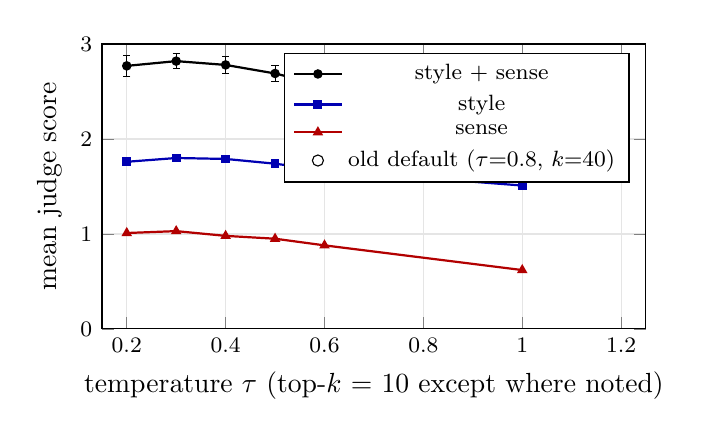
\begin{tikzpicture}
\begin{axis}[
  width=0.7\textwidth, height=5.2cm,
  xlabel={temperature $\tau$ (top-$k$ = 10 except where noted)},
  ylabel={mean judge score},
  xmin=0.15, xmax=1.25, ymin=0, ymax=3,
  grid=major, grid style={gray!20}, tick label style={font=\footnotesize},
  legend style={font=\footnotesize, at={(0.97,0.97)}, anchor=north east}]
\addplot[thick, black, mark=*, mark size=1.3pt, error bars/.cd, y dir=both, y explicit]
  coordinates {(0.2,2.77)+-(0,0.11) (0.3,2.82)+-(0,0.08) (0.4,2.78)+-(0,0.09) (0.5,2.69)+-(0,0.08)
               (0.6,2.56)+-(0,0.07) (1.0,2.13)+-(0,0.07)};
\addlegendentry{style + sense}
\addplot[thick, blue!70!black, mark=square*, mark size=1.2pt]
  coordinates {(0.2,1.76)(0.3,1.80)(0.4,1.79)(0.5,1.74)(0.6,1.67)(1.0,1.51)};
\addlegendentry{style}
\addplot[thick, red!70!black, mark=triangle*, mark size=1.4pt]
  coordinates {(0.2,1.01)(0.3,1.03)(0.4,0.98)(0.5,0.95)(0.6,0.88)(1.0,0.62)};
\addlegendentry{sense}
\addplot[only marks, mark=o, mark size=2pt] coordinates {(0.8,2.23)};
\addlegendentry{old default ($\tau{=}0.8$, $k{=}40$)}
\end{axis}
\end{tikzpicture}
\caption{Judged quality falls steadily as temperature rises, so the default
moved to $\tau = 0.4$, $k = 10$ (3.2M model; error bars $\pm$ one standard error).
Below $0.4$ the model begins to loop, which the judge barely penalizes, so
diversity (distinct 4-grams, $0.95$ at $\tau = 0.4$) sets the lower bound.}
\label{fig:tune}
\end{figure}

\subsection{Looking inside}

\begin{description}
  \item[Attention] For each layer and head the Lab shows the matrix
        $A^{(\ell, j)} = \softmax\bigl(Q_j K_j^\top/\sqrt{d_h} + M\bigr) \in \R^{T\times T}$
        from \cref{eq:attn}.
  \item[Logit lens] The residual stream after layer $\ell$ is decoded with the
        final norm and the tied head, as if the network stopped there
        \cite{logitlens}:
        $\hat{\bm{p}}^{(\ell)}_t = \softmax\bigl(W_{\text{tok}}\LN_f(\bm{h}^{(\ell)}_t)\bigr)$
        for $\ell = 0, \dots, N_L$. The Lab lists the top three characters per
        position and layer, so the user can watch the guess form.
  \item[Surprise] Each real verse $v$ of $n_v$ characters is scored by its mean
        per-character loss,
        $\operatorname{surprise}(v) = -\frac{1}{n_v}\sum_{t=1}^{n_v}\log \Pr_{\bm\theta}(x_t \mid x_{<t})$,
        with perplexity $e^{\operatorname{surprise}(v)}$. This ranks the verses
        the model finds least predictable by its own statistics.
\end{description}

\section{Memorization: the FSRS scheduler}\label{sec:fsrs}

Verses learned by heart are scheduled with FSRS-4.5 \cite{fsrs}, using its
published default weights $w_0, \dots, w_{16}$. A memory has a stability $S$, the
interval in days at which recall falls to $90\%$, and a difficulty
$D \in [1, 10]$. The probability of recall after $t$ days is the power-law
forgetting curve
\begin{equation}\label{eq:retrievability}
  R(t, S) = \left(1 + \frac{19}{81}\cdot\frac{t}{S}\right)^{-1/2},
\end{equation}
where the factor $19/81$ makes $R(S, S) = 0.9$ exactly. The next interval for
target retention $R^\ast = 0.9$ solves $R(I, S) = R^\ast$:
\begin{equation}
  I(S) = \max\!\left(1,\; \operatorname{round}\!\left[\frac{81}{19}\,S\left((R^\ast)^{-2} - 1\right)\right]\right) = \max(1, \operatorname{round}(S)).
\end{equation}
For a review with grade $g \in \{1, 2, 3, 4\}$ (again, hard, good, easy) at
current recall $R$ from \cref{eq:retrievability}, writing
$D_0(g) = w_4 - e^{w_5(g-1)} + 1$:
\begin{align}
  D' &= \operatorname{clip}_{[1,10]}\!\Bigl(w_7\,D_0(4) + (1 - w_7)\bigl(D - w_6(g - 3)\bigr)\Bigr), \\
  S'_{\text{recall}} &= S\left(1 + e^{w_8}\,(11 - D')\,S^{-w_9}\left(e^{w_{10}(1-R)} - 1\right) h_g\, b_g\right), \\
  S'_{\text{lapse}} &= w_{11}\, (D')^{-w_{12}}\left((S+1)^{w_{13}} - 1\right) e^{w_{14}(1-R)},
\end{align}
with the hard penalty $h_2 = w_{15}$, the easy bonus $b_4 = w_{16}$, and
$h_g = b_g = 1$ otherwise. A first review sets $S = w_{g-1}$ and $D = D_0(g)$. A
lapse ($g = 1$) uses $S'_{\text{lapse}}$, and the card returns in ten minutes.

\section{Halftoning}\label{sec:halftone}

Illustrations behind the interface are reduced to one bit per pixel at their
drawn size. The image is first converted to grey with luma weights,
$Y = 0.299R + 0.587G + 0.114B$, and its 1st and 99th percentiles are stretched
to black and white. Let $I(x, y) \in [0, 255]$ be the result and
$\hat{I} \in \{0, 255\}$ the output; a pixel is inked when it falls below its
threshold.

\paragraph{Error diffusion.} Each pixel is thresholded at $128$, and its error
$\epsilon = I - \hat{I}$ is pushed to unvisited neighbours. Floyd--Steinberg
\cite{floyd} distributes all of it and runs in serpentine order (alternate rows
right to left, with the kernel mirrored). Atkinson distributes $6/8$, which keeps
highlights and shadows crisp:
\begin{equation}
  \text{FS: } \frac{1}{16}\begin{bmatrix} & \ast & 7 \\ 3 & 5 & 1 \end{bmatrix},
  \qquad
  \text{Atkinson: } \frac{1}{8}\begin{bmatrix} & \ast & 1 & 1 \\ 1 & 1 & 1 & \\ & 1 & & \end{bmatrix}.
\end{equation}

\paragraph{Ordered dithering.} An $8 \times 8$ Bayer matrix, the $n = 8$ case of
the recurrence
\begin{equation}
  B_{2n} = \begin{bmatrix} 4B_n & 4B_n + 2 \\ 4B_n + 3 & 4B_n + 1 \end{bmatrix},
  \qquad B_1 = [0],
\end{equation}
sets the threshold $255\,\bigl(B_8[x \bmod 8, y \bmod 8] + \tfrac12\bigr)/64$.

\paragraph{Blue noise.} A void-and-cluster threshold array \cite{ulichney}
replaces $B_8$, with thresholds $255\,(\operatorname{rank} + \tfrac12)/N$ for the
$N$ cells of the tile. Clusters and voids are located with a toroidal Gaussian
energy of radius $5$ and $\sigma = 1.5$,
\begin{equation}
  \mathcal{E}(p) = \sum_{q \,:\, \text{ink}} \exp\!\left(-\frac{\lVert p - q\rVert^2}{2\sigma^2}\right),
\end{equation}
which gives a pattern with no low-frequency structure, so it shows none of the
crosshatch of a Bayer grid.

\section{Limitations}\label{sec:limits}

\begin{description}
  \item[Recall ceiling] With a top-$20$ candidate list, $9$ of $30$ benchmark
        questions have no relevant verse to promote. Passage-level embeddings or
        a larger candidate set before reranking would raise recall.
  \item[Benchmark size] Thirty questions with binary labels support a
        direction, not a precise effect size.
  \item[Model ceiling] At every sampling setting, judged sense stays near $1$
        of $3$. That limit is the model's (depth, context, training steps), not
        the sampler's.
  \item[ELS on English] The Bible-codes lesson runs on the English KJV rather
        than the Hebrew text, so it illustrates the statistics, not the
        original claim.
\end{description}

\section*{Preparation}

This paper was drafted with an AI assistant (Claude) from the project's source
code and documentation and checked against them; the author is responsible for
its content. \Cref{app:provenance} lists the source of every number.

\begin{thebibliography}{99}
\bibitem{bge} S.~Xiao, Z.~Liu, P.~Zhang and N.~Muennighoff. C-Pack: Packaged
  resources to advance general Chinese embedding. arXiv:2309.07597, 2023.
\bibitem{rrf} G.~V. Cormack, C.~L.~A. Clarke and S.~Buettcher. Reciprocal rank
  fusion outperforms Condorcet and individual rank learning methods. In
  \emph{SIGIR}, 2009.
\bibitem{acl} R.~Andersen, F.~Chung and K.~Lang. Local graph partitioning using
  PageRank vectors. In \emph{FOCS}, 2006.
\bibitem{leiden} V.~A. Traag, L.~Waltman and N.~J. van Eck. From Louvain to
  Leiden: guaranteeing well-connected communities. \emph{Scientific Reports},
  9:5233, 2019.
\bibitem{burrows} J.~Burrows. \enquote{Delta}: a measure of stylistic difference
  and a guide to likely authorship. \emph{Literary and Linguistic Computing},
  17(3):267--287, 2002.
\bibitem{gpt2} A.~Radford, J.~Wu, R.~Child, D.~Luan, D.~Amodei and I.~Sutskever.
  Language models are unsupervised multitask learners. OpenAI, 2019.
\bibitem{adamw} I.~Loshchilov and F.~Hutter. Decoupled weight decay
  regularization. In \emph{ICLR}, 2019.
\bibitem{logitlens} nostalgebraist. Interpreting GPT: the logit lens.
  LessWrong, 2020.
\bibitem{fsrs} J.~Ye, J.~Su and Y.~Cao. A stochastic shortest path algorithm
  for optimizing spaced repetition scheduling. In \emph{KDD}, 2022.
\bibitem{floyd} R.~W. Floyd and L.~Steinberg. An adaptive algorithm for spatial
  greyscale. \emph{Proceedings of the SID}, 17(2):75--77, 1976.
\bibitem{ulichney} R.~Ulichney. The void-and-cluster method for dither array
  generation. In \emph{Proc.\ SPIE 1913}, 1993.
\end{thebibliography}

\appendix
\section{Provenance of numbers}\label{app:provenance}

\begin{table}[htbp]
\centering
\caption{Where each reported number comes from. Paths are relative to the
\code{biblelm} repository; \code{data/} means \code{public/data/}, the local
build output, which is not committed.}
\label{tab:provenance}
\small
\begin{tabular}{>{\raggedright\arraybackslash}p{0.42\textwidth} >{\raggedright\arraybackslash}p{0.52\textwidth}}
\toprule
Number & Source \\
\midrule
$M = 39{,}904$, dimension $384$, scale $s = 400$ & \code{data/embeddings.json}; index size from \code{data/embeddings.i8} \\
CLS pooling, normalization, int8 clipping & \code{scripts/data/embed.mjs} \\
Smoothing weights, top-$k$, interpolation, chiasm matrix & \code{src/lib/semantic.worker.ts}, \code{semantic.ts} \\
RRF $k = 60$; topic cap $20$ & \code{src/lib/semantic.ts} (\code{fuse}); \code{docs/ML.md} \\
Reranking metrics and counts & \code{docs/evals/shadow.md} \\
$\alpha$, $\varepsilon$, limit, push cap; Dijkstra cost & \code{src/lib/xrefs.ts} \\
About $341{,}000$ cross references; Louvain $\gamma = 12$ & \code{README.md}; \code{docs/IDEAS.md} \\
tf-idf, PMI window, Zipf ranks, Delta $F = 150$ & \code{src/lib/words.ts} \\
ELS skips and null model & \code{src/lib/els.ts} \\
GPT shape, defaults, optimizer, clipping & \code{python/biblelm/model.py}, \code{train.py}, \code{tokenizer.py} \\
Logit lens top $3$, surprise & \code{python/biblelm/inspect\_model.py} \\
Validation loss $1.224$, sampling study & \code{docs/evals/tuning.md} \\
FSRS weights and formulas & \code{src/lib/fsrs.ts} \\
Grey conversion, kernels, Bayer and blue-noise thresholds & \code{src/art/dither.ts} \\
Derived: index bytes, parameter counts, bits per character, nDCG ceiling & computed from the rows above \\
\bottomrule
\end{tabular}
\end{table}

\paragraph{Not confirmed.} The repository documents state $37{,}885$ indexed
verses, while the local build holds $39{,}904$; this paper uses the build. The
vocabulary size $V$ depends on the training corpus and no trained run is present
locally, so parameter counts are given as functions of $V$.

\end{document}
